\section{Transient Absorption}
\label{sec:TRAS}


\begin{table}[ht]
    \centering
    \begin{tabular}{clc}
        \toprule
        Sample No. &    Treatment &    $\tau$ / \si{\nano\second} \\
        \midrule
        1 &     ZnTPP in bn 0.8mM &  $953 \pm 3$ \\
        2 &     ZnTPP in bn 0.6mM &  $972 \pm 4$ \\
        3 &     ZnTPP in bn 0.4mM & $1000 \pm 4$ \\
        4 &     ZnTPP in bn 0.2mM & $1008 \pm 8$ \\
        5 & ZnTPP:C70 in bn 1:0.1 &  $834 \pm 3$ \\
        6 & ZnTPP:C70 in bn 1:0.2 &  $753 \pm 3$ \\
        7 & ZnTPP:C70 in bn 1:0.3 &  $697 \pm 3$ \\
        8 &    ZnTPP in tol 0.8mM &  $533 \pm 1$ \\
        12 &     ZnOEP in bn 0.8mM &  $373 \pm 1$\\
        \bottomrule
    \end{tabular}
\end{table}



\subsection*{Variation in Concentration}
For ZnTPP, different concentrations in bn were measured. From the theory, we expect an exponential decay of the concentration of the triplet 
\begin{equation}
    C_T(t) = C_T(0) \exp[-k_0t],
\end{equation}
with the initital concentration $C_T(0)$ and the decay rate $k_0$.
As the transient absorption $\Delta A(\tau)$ is proportional to $C_T$, we can fit an exponential decay to our data. Hereby, an offset was added to the decay function to correct any offset caused by e.g.~measuring methods. Data and fits are shown in fig.~\ref{fig:TRAS-Conc}.

\begin{figure}[h]
    \centering
    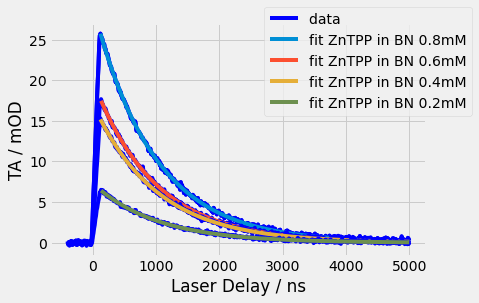
\includegraphics[width = 0.9\textwidth]{Bilder/Auswertung/TRAS/ZnTPPdiffConc.png}
    \caption{Data of the transient absorption of solutions of different concentrations of ZnTPP in bn.}
    \label{fig:TRAS-Conc}
\end{figure}

It is clear, that higher maxima correspond to higher concentrations of ZnTPP. This aligns our expectations as a higher concentration leads to a bigger ammount of absorption. The lifetime $\tau_0$ can be calculated from 
\begin{equation}
    \tau_0 = \frac{1}{k_0}.
\end{equation}

The calculated lifetimes can be found in tab.~\ref{tab:lifetimesConc}.

\begin{table}[ht]
    \centering
    \begin{tabular}{clc}
        \toprule
        Sample No. &    Treatment &    $\tau$ / \si{\nano\second} \\
        \midrule
        1 &     ZnTPP in bn 0.8mM &  $953 \pm 3$ \\
        2 &     ZnTPP in bn 0.6mM &  $972 \pm 4$ \\
        3 &     ZnTPP in bn 0.4mM & $1000 \pm 4$ \\
        4 &     ZnTPP in bn 0.2mM & $1008 \pm 8$ \\
        \bottomrule
    \end{tabular}
    \caption{Calculated lifetimes of ZnTPP solutions in bn with different concentrations.}
    \label{tab:lifetimesConc}
\end{table}

Here, an increasing lifetime for decreasing concentrations of ZnTPP is evident. This aligns our expectations from theory: The kinetics of the decay of the triplet state are determined by the differential equation 
\begin{equation}
    \frac{dC_T(t)}{dt} = - k_1C_T(t) - k_2(C_T(t))^2 - k_3 C_T(t)C_G(t),
\end{equation}
where $C_{T/G}(t)$ is the concentration of the triplet/ground state and $k_{1/2/3}$ are decay rates. In general the assumption is made, that $C_T(t) \ll C_G(t)$, which eventually leads to the exponential decay. However, the decay rate is therefore always underestimated as one process is neglected. Furthermore, the assumption becomes less valid, with an increasing population of the triplet state. Thus, we expect higher decay rates (i.e.~shorter lifetimes) for an increasing concentration of triplet states, which we assigned above to the higher concentrations of ZnTPP. In this way, the decreasing lifetimes for increasing concentrations of ZnTPP can be explained.

\subsection*{Quenching with C\textsubscript{70}}
The lifetime of a triplett state can be reduced by allowing further decay paths. In this experiment, this was achieved by adding different concentrations of the fullerene C\textsubscript{70} to the ZnTPP solutions of \SI{0.8}{\milli\nauticalmile} concentration (solvent:bn). The data and corresponding fits can be seen in fig.~\ref{fig:ZnTPP-C70}. The reduced population of the triplet state for an increasing concentration of fullerene can be seen as an decrease of the maximum transient absorption. The lifetimes can be calculated as shown above. They and the corresponding decay rates are displayed in tab.~\ref{tab:ZnTPP-C70}. As expected, the lifetime decreases with an increasing ammount of fullerene due to more quanching processes being able. 

\begin{figure}[h]
    \centering
    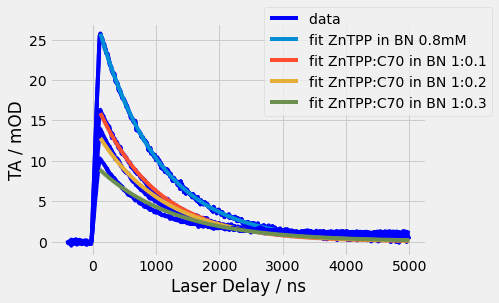
\includegraphics[width = 0.9\textwidth]{Bilder/Auswertung/TRAS/ZnTPP-C70.png}
    \caption{Data of the transient absorption of different dillutions of C\textsubscript{70} in \SI{0.8}{\milli\nauticalmile} ZnTPP in bn.}
    \label{fig:ZnTPP-C70}
\end{figure}

\begin{table}[ht]
    \centering
    \begin{tabular}{clcc}
        \toprule
        Sample No. &    Treatment & $k_{app}$ / \si{\per\milli\second}  &  $\tau$ / \si{\nano\second} \\
        \midrule
        1 &     ZnTPP in bn 0.8mM & $1050 \pm 3$ &  $953 \pm 3$ \\
        5 & ZnTPP:C70 in bn 1:0.1 & $1198 \pm 4$ &  $834 \pm 3$ \\
        6 & ZnTPP:C70 in bn 1:0.2 & $1329 \pm 5$ &  $753 \pm 3$ \\
        7 & ZnTPP:C70 in bn 1:0.3 & $1436 \pm 6$ &  $697 \pm 3$ \\
        \bottomrule
    \end{tabular}
    \caption{Calculated lifetimes of different dillutions of fullerene C\textsubscript{70} in a \SI{0.8}{\milli\nauticalmile} solution in bn.}
    \label{tab:ZnTPP-C70}
\end{table}

To determine the rate of the quenching process $k_q$, the decay rates of the different dillutions $k_{app}$ are plotted against the concentrations of fullerene $[C_{70}]$. Since $k_{app}$ was defined as 
\begin{equation}
    k_{app} = k_0 + k_q C_q,
\end{equation}
$k_q$ corresponds to the slope of the line, which is fitted in fig.~\ref{fig:C70-kq}. A quenching rate of \par 
\centerline{\boxed{k_q =  \SI{1.61 \pm 0.08}{\per\micro\second\per\milli\nauticalmile}}} \par 
was determined. This value does not completely align with the values found by Ito et al., who determined $k_q = $\SI{4.7}{\per\micro\second\per\milli\nauticalmile}~\cite{Nojiri.1998}. Though, the error is within one order of magnitude. 

\begin{figure}[h]
    \centering
    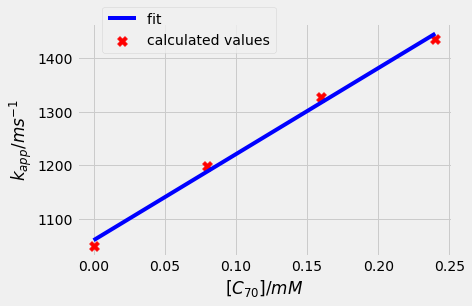
\includegraphics[width = 0.9\textwidth]{Bilder/Auswertung/TRAS/ZnTPP-C70-kq.png}
    \caption{Data of the transient absorption of different dillutions of C\textsubscript{70} in \SI{0.8}{\milli\nauticalmile} ZnTPP in bn.}
    \label{fig:C70-kq}
\end{figure}

%#kyliewarhier

\subsection*{Change of solvent}

In the case of \SI{0.8}{\milli\nauticalmile} ZnTPP, solutions with two different solvents were measured (bn and tol). Analagous to the recent evaluation, the the transient absorption is shown in fig.~\ref{fig:ZnTPP-bn-tol} and the lifetimes were calculated via an exponential decay fit (see tab.~\ref{fig:ZnTPP-bn-tol}).

\begin{figure}[h]
    \centering
    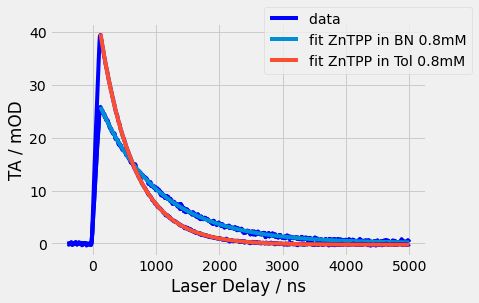
\includegraphics[width = 0.9\textwidth]{Bilder/Auswertung/TRAS/ZnTPP-bn-tol.png}
    \caption{Data of the transient absorption of \SI{0.8}{\milli\nauticalmile} ZnTPP in bn and in tol. For tol a higher maximum transient absorption value was measured.}
    \label{fig:ZnTPP-bn-tol}
\end{figure}


\begin{table}[ht]
    \centering
    \begin{tabular}{clc}
        \toprule
        Sample No. &    Treatment &    $\tau$ / \si{\nano\second} \\
        \midrule
        1 &     ZnTPP in bn 0.8mM &  $953 \pm 3$ \\
        8 &    ZnTPP in tol 0.8mM &  $533 \pm 1$ \\
        \bottomrule
    \end{tabular}
    \caption{Calculated lifetimes of \SI{0.8}{\milli\nauticalmile} ZnTPP solutions in bn and tol.}
    \label{tab:ZnTPP-bn-tol}
\end{table}